
\section{CPU architecture}

The Central Processing Unit (CPU) is the main processing unit within a
computer. 

The CPU contains both :
\begin{itemize}
    \item the {\bf Control Unit (CU)}in charge of moving and controlling data
    \item the {\bf Arithmetic/Logic Unit (ALU)}in charge of performing various
        arithmetics and logical calculations as requested by a program through
        the assembly instructions.
\end{itemize}

The manner in which and how efficiently a CPU processes its instructions
depends on its {\bf Instruction Set Architecture (ISA)}. There are multiple
ISA's in the industry, each having its way of processing data:
\begin{itemize}
    \item {\bf RISC} architecture: ased on processing more simple instructions, which takes more cycles, but each cycle is shorter and takes less power. 
    \item {\bf CISC} architecture is based on fewer, more complex instructions, which
        can finish the requested instructions in fewer cycles, but each
        instruction takes more time and power to be processed.
\end{itemize}

\subsection{Clock Speed \& Clock Cycle}

Each CPU has a clock speed that indicates its overall speed. Every tick of the
clock runs a clock cycle that processes a basic instruction, such as fetching
an address or storing an address. Specifically, this is done by the CU or AU.

The frequency in which the cycles occur is counted is cycles per second
(Hertz). If a CPU has a speed of 3.0 GHz, it can run 3 billion cycles every
second (per core).

 \begin{figure}
  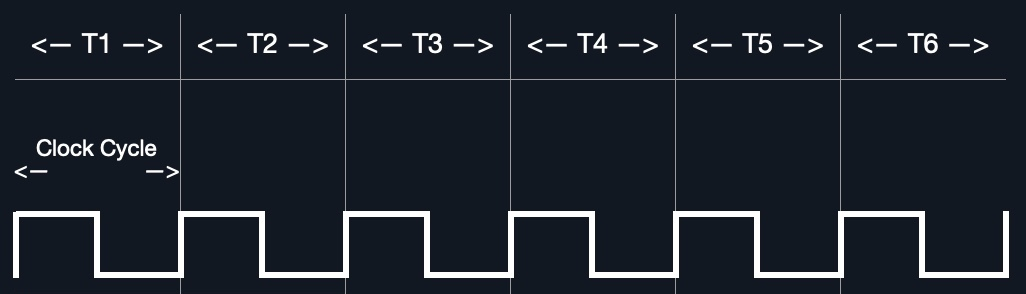
\includegraphics[width=\linewidth]{binary/intro/images/assembly_clock_cycle_0.jpg}
  \caption{Clock cycle}
  \label{fig:clock_cycle_O}
\end{figure}

Modern processors have a multi-core design, allowing them to have multiple
cycles at the same time.


\subsection{Instruction Cycle}
An Instruction Cycle is the cycle it takes the CPU to process a single machine
instruction. An instruction cycle consists of four stages:
\begin{itemize}
    \item Fetch: Takes the next instruction's address from the {\bf Instruction
        Address Register (IAR)}.
    \item Decode: Takes the instruction from the IAR, and decodes it from
        binary to see what is required to be executed.
    \item Execute: Fetch instruction operands from register/memory, and process
        the instruction in the ALU or CU.
    \item Store: Store the new value in the destination operand.
\end{itemize}

Each Instruction Cycle takes multiple clock cycles to finish, depending on the
CPU architecture and the complexity of the instruction. Once a single
instruction cycle ends, the CU increments to the next instruction and runs the
same cycle on it, and so on.

 \begin{figure}
  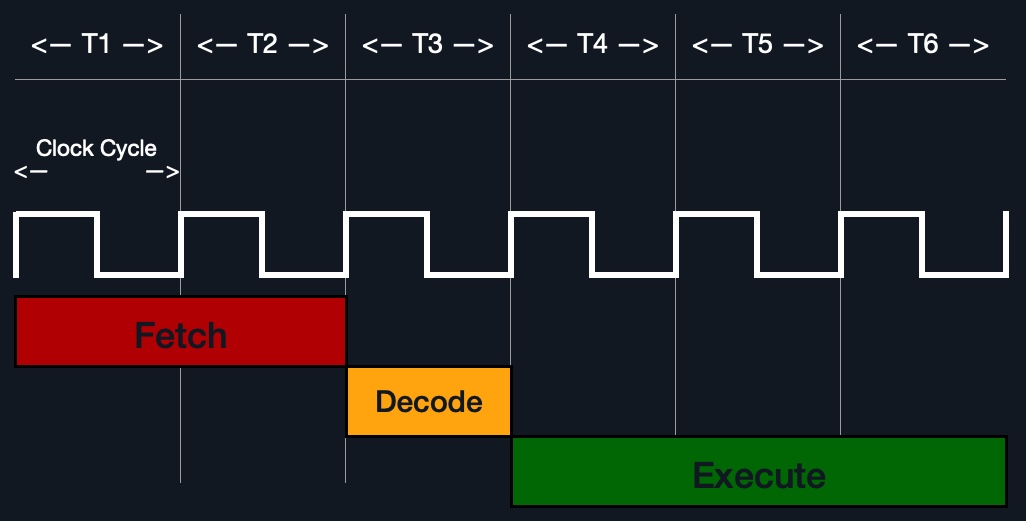
\includegraphics[width=\linewidth]{binary/intro/images/assembly_clock_cycle_1.jpg}
  \caption{Instruction cycle}
  \label{fig:clock_cycle_1}
\end{figure}


In the past, processors used to process instructions sequentially, so they had
to wait for one instruction to finish to start the next. On the other hand,
modern processors can process multiple instructions in parallel by having
multiple instruction/clock cycles running at the same time. This is made
possible by having a multi-thread and multi-core design.

 \begin{figure}
  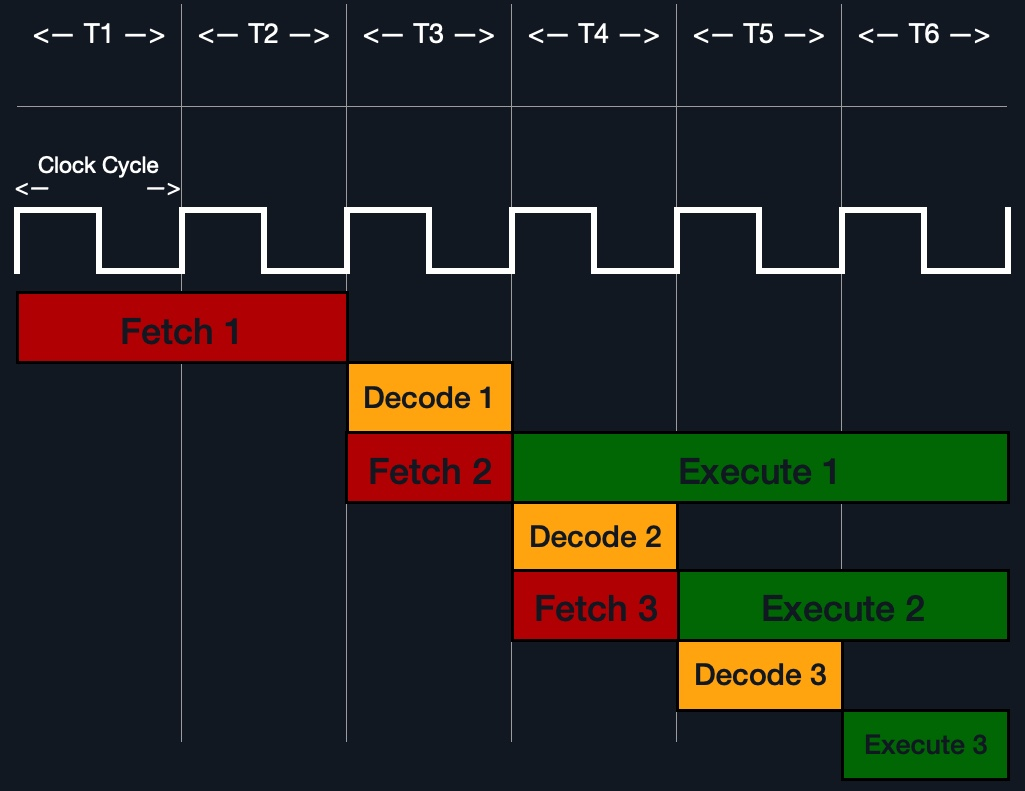
\includegraphics[width=\linewidth]{binary/intro/images/assembly_clock_cycle_2.jpg}
  \caption{Multi-thread instruction cycle}
  \label{fig:clock_cycle_2}
\end{figure}

\subsection{Processor Specific}

Each processor type has a different low-level assembly language
architecture known as {\bf Instruction Set Architectures (ISA)}.

Furthermore, a single Instruction Set Architecture may have several syntax
interpretations for the same assembly code. The instruction written as
\verb+add rax, 1+ with Intel syntax, and written as \verb+addb $0x1,%rax+ with
AT\&T syntax.

As we can see, even though we can tell that both instructions are similar and
do the same thing, their syntax is different, and the locations of the source
and destination operands are swapped as well. Still, both codes assemble the
same machine code and perform the same instruction.



So, each processor type has its Instruction Set Architectures, and each
architecture can be further represented in several syntax formats.

in linux \verb+lscpu+ provide information on the the architecture:
\begin{verbatim}
$ lscpu

Architecture:                    x86_64
CPU op-mode(s):                  32-bit, 64-bit
Byte Order:                      Little Endian

<SNIP>
\end{verbatim}

As we can see in the above output, the CPU architecture is \verb+x86_64+, and
supports 32-bit and 64-bit. The byte order is {\bf Little Endian}. 

